\documentclass{article}
\usepackage{graphicx}
\usepackage[hidelinks]{hyperref}
\usepackage{float}
\usepackage[utf8]{inputenc}
\usepackage[spanish]{babel}
\usepackage{csquotes}
\usepackage{listings}
\usepackage[a4paper, left=3cm, right=2.5cm, top=3cm, bottom=3cm]{geometry}
\usepackage{fancyhdr}
\usepackage{lastpage}
\usepackage{minted}
\usepackage{tikz}
\usepackage{xcolor}
\usepackage[bottom]{footmisc}
\usepackage{booktabs}
\usepackage{pdflscape}
\usepackage{adjustbox}
\usepackage[backend=biber, style=numeric]{biblatex}
\usepackage{bookmark}

% Configuración de la bibliografía
\addbibresource{references.bib}

% Definición de nuevos comandos
\newcommand{\mail}[2]{\href{mailto:#1}{#2}}
\definecolor{mygreen}{RGB}{124, 180, 76}
\definecolor{mycyan}{RGB}{100, 124, 204}

\pagestyle{fancy}
\fancyhf{}
 
\fancyfoot[R]{Página \thepage\ de \pageref{LastPage}}

% Definir un estilo para las páginas landscape con "Página X de Y" alineado a la derecha sin negrita
\fancypagestyle{landscape}{
  \fancyhf{}  % Limpiar encabezado y pie de página
  \fancyfoot{%
    \tikz[remember picture,overlay]
      \node[outer sep=2cm,above,rotate=90] at (current page.east) {Página \thepage\ de \pageref{LastPage}};}
}

\setlength{\parindent}{0pt}

\renewcommand{\headrulewidth}{0pt}
\renewcommand{\footrulewidth}{0pt}

\lstset{
    basicstyle=\ttfamily, % Estilo monoespaciado para el código
    breaklines=true,      % Romper líneas largas automáticamente
    breakatwhitespace=true, % Romper líneas largas en espacios
}

\graphicspath{{images/}}

\definecolor{highlightcolor}{rgb}{1.0, 0.76, 0.0}
\definecolor{bgcolor}{rgb}{0.95, 0.95, 0.95}

% Definición de la portada del documento
\title{
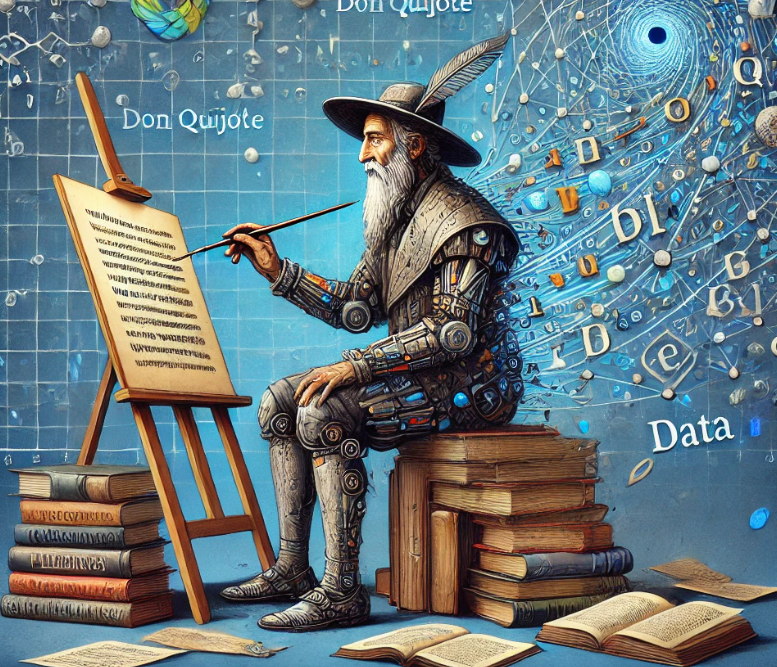
\includegraphics[scale=0.5]{don_quijote_generativo.png} \\
\vspace{2em}
\textbf{Deep Learning} \\ \rule{0.8\textwidth}{0.5pt} \\ \large \textbf{Programación de Bases de Datos}}
\author{Daniel Torres Galindo \thanks{dtorrescb@alumnos.unex.es} \and Daniel Sánchez Parra \thanks{dsanchezfe@alumnos.unex.es}}
\date{\today}

% Cambiar el formato de los números de las notas a pie de página
\makeatletter
\let\@fnsymbol\@arabic
\makeatother

\begin{document}

\maketitle

\thispagestyle{empty}

\begin{figure}[H]
    \centering
    
\includegraphics[width=0.7\textwidth]{logo-uex.png}
\end{figure}

% Línea de pie de página de la portada
\renewcommand{\footnoterule}{
    \vspace{1em}
    \hrule width \linewidth height 0.5pt
    \vspace{0.5em}
}

\newpage

\tableofcontents

\newpage

\section{Introducción}
\subsection{Contexto y objetivo del proyecto}
En un mundo donde el procesamiento del lenguaje natural (NLP, por sus siglas en inglés) está revolucionando la forma en que interactuamos con la tecnología, el desarrollo de modelos capaces de generar texto de manera autónoma se ha convertido en un tema clave.
Desde asistentes virtuales como Siri y Alexa hasta herramientas avanzadas de escritura asistida, los sistemas de generación de texto están transformando industrias enteras. \\

El presente proyecto busca explorar esta tecnología utilizando una obra literaria clásica, \textbf{Don Quijote de la Mancha}, como conjunto de datos base.
A través del uso de Redes Neuronales Recurrentes (RNN), especialmente diseñadas para manejar datos secuenciales, pretendemos imitar el estilo de escritura de Miguel de Cervantes, generando texto carácter por carácter.
Este enfoque no solo pone a prueba la capacidad del modelo para capturar dependencias complejas en el lenguaje, sino que también muestra cómo las técnicas de Deep Learning pueden aplicarse en dominios creativos. \\

\subsection{Objetivos específicos}

\begin{itemize}
    \item \textbf{Preparación de Datos}: Descargar, preprocesar y tokenizar el texto de \emph{Don Quijote de la Mancha} para convertirlo en un formato adecuado para entrenamiento de modelos.
    \item \textbf{Diseño del Modelo}: Construir una arquitectura basada en RNN que incluya capas de embeddings, LSTM, y una capa de salida para predicción carácter por carácter.
    \item \textbf{Entrenamiento}:
    \begin{itemize}
        \item Ajustar hiperparámetros como tamaño del batch, número de épocas y función de pérdida.
        \item Implementar un proceso de entrenamiento eficiente que permita capturar las dependencias a largo plazo presentes en el texto.
    \end{itemize}
    \item \textbf{Generación de Texto}:
    \begin{itemize}
        \item Utilizar el modelo entrenado para generar texto de forma iterativa, ajustando la temperatura para variar la creatividad en las predicciones.
    \end{itemize}
    \item \textbf{Evaluación}:
    \begin{itemize}
        \item Analizar los textos generados, comparándolos con el estilo literario del texto original.
        \item Evaluar la coherencia, fluidez y calidad del texto generado.
    \end{itemize}
\end{itemize}

\subsection{Justificación del uso de RNN en generación de texto}
Las redes neuronales recurrentes (RNN) son un tipo de red neuronal que se utiliza comúnmente en tareas de procesamiento del lenguaje natural, como la generación de texto. Son capaces de modelar dependencias temporales en los datos, lo que las hace especialmente adecuadas para tareas en las que la secuencia de los datos es importante.
En el caso de la generación de texto, estas son capaces de capturar la estructura y el estilo del texto original, lo que les permite generar texto coherente y similar al original. Por esta razón, las (RNN) son una elección natural para este tipo de tarea.

\newpage

\section{Marco Teórico}
\subsection{Introducción al Deep Learning}
El Deep Learning es una rama del aprendizaje automático que se basa en el uso de redes neuronales artificiales para modelar y aprender patrones en los datos.
Las redes neuronales artificiales son modelos matemáticos inspirados en el funcionamiento del cerebro humano, que consisten en capas de neuronas interconectadas que se utilizan para procesar y aprender a partir de los datos. \\

El Deep Learning se ha convertido en una herramienta poderosa para una amplia variedad de aplicaciones, incluido el procesamiento del lenguaje natural, la visión por computador y la generación de texto.

\begin{figure}[H]
    \centering
    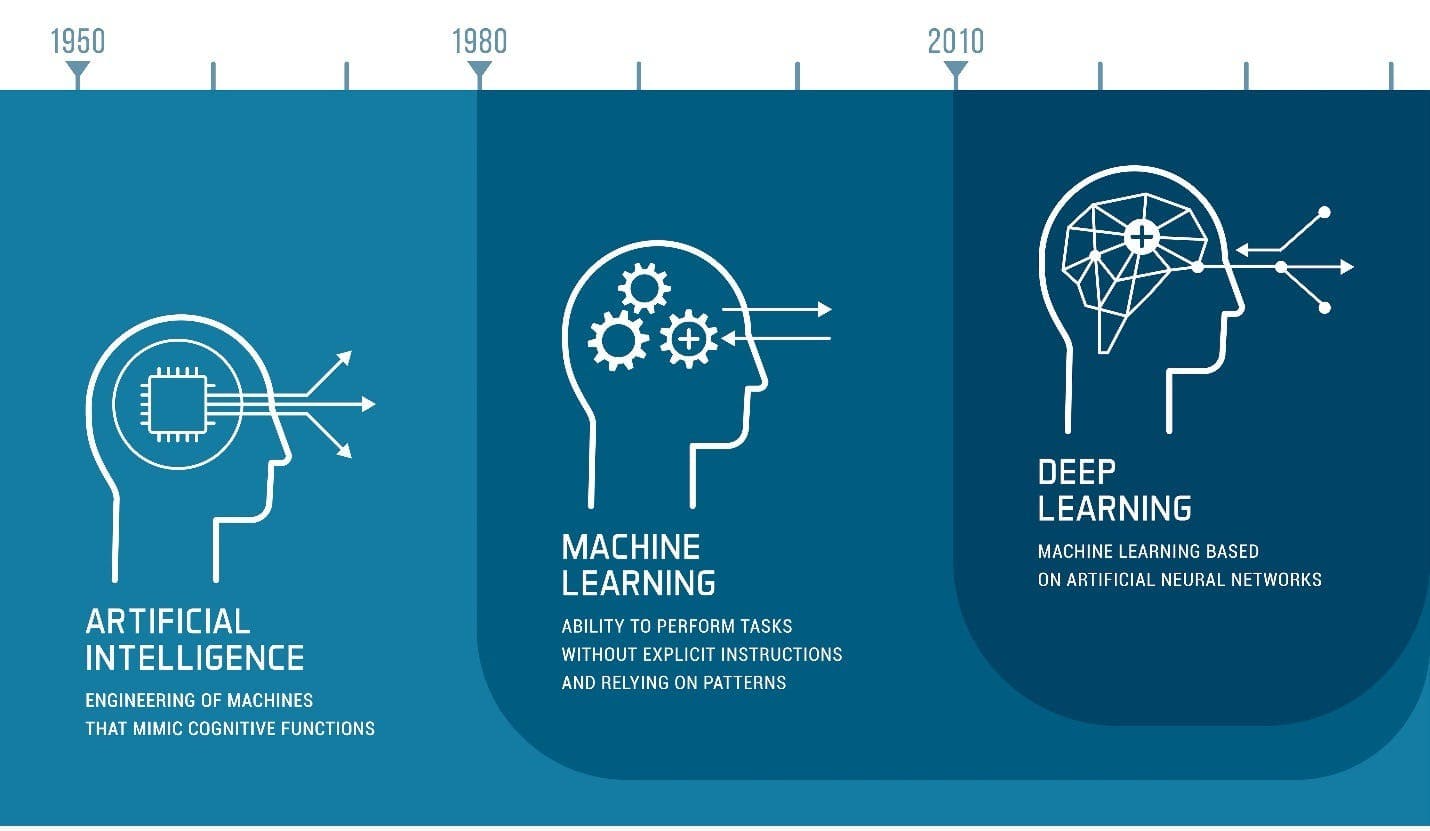
\includegraphics[scale=0.2]{history.png}
    \caption{Cronograma sobre el avance de la Inteligencia Artificial. \cite{tjk2024deep}}
\end{figure}

\subsubsection{Fundamentos del Deep Learning}

\subsubsection{Aplicaciones del Deep Learning}
Las aplicaciones del Deep Learning son variadas y abarcan campos como el procesamiento del lenguaje natural, la visión por computador, la generación de texto, la traducción automática, entre otros.

\newpage

\subsection{Redes Neuronales Recurrentes (RNN)}
\subsubsection{¿Qué son las RNN?}
Una red neuronal recurrente, o (RNN), es una red neuronal \cite{ibm-nn} profunda entrenada con datos secuenciales o de series temporales para crear un modelo de machine learning \cite{ibm-ml} que pueda hacer predicciones secuenciales o conclusiones basadas en entradas secuenciales. \\

Una (RNN) podría utilizarse para predecir los niveles diarios de inundación basándose en los datos diarios anteriores sobre inundaciones, mareas y meteorología.
Pero las (RNN) también se pueden utilizar para resolver problemas ordinales o temporales, como la traducción de idiomas, el procesamiento del lenguaje natural (PLN) \cite{ibm-pln}, el reconocimiento de voz \cite{ibm-sr} y el subtitulado de imágenes.
Las (RNN) se incorporan a aplicaciones populares como Siri, búsqueda por voz y Google Translate.

\subsubsection{Funcionamiento de las RNN}
Al igual que [las redes neuronales convolucionales CNN \cite{ibm-cnn}, las redes neuronales recurrentes utilizan datos de entrenamiento para aprender.
Se distinguen por su ``memoria'', ya que toman la información de las entradas anteriores para influir en la entrada y la salida actuales.
Aunque las redes neuronales profundas tradicionales asumen que las entradas y las salidas son independientes entre sí, la salida de los (RNN) depende de los elementos anteriores de la secuencia.
Mientras que las redes neuronales profundas tradicionales asumen que las entradas y las salidas son independientes entre sí, la salida de las (RNN) depende de los elementos anteriores dentro de la secuencia. \\

Tomemos un modismo, como el inglés ``feeling under the weather'', que se utiliza comúnmente cuando alguien está enfermo, para ayudarnos en la explicación de las (RNN).
Para que el modismo tenga sentido, debe expresarse en ese orden específico.
En consecuencia, las redes recurrentes deben tener en cuenta la posición de cada palabra en el modismo y utilizan esa información para predecir la siguiente palabra de la secuencia.

\begin{figure}[H]
    \centering
    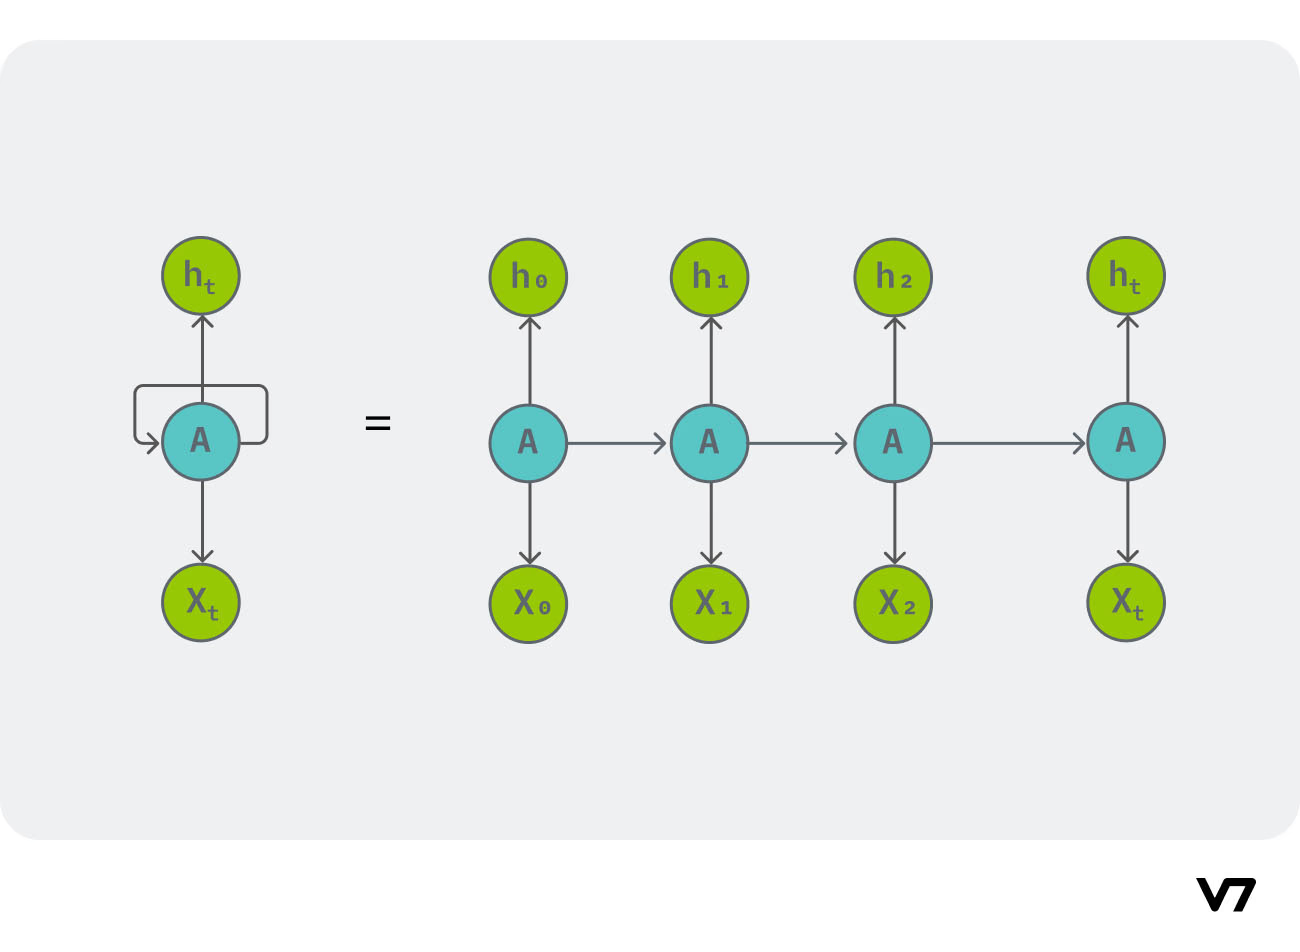
\includegraphics[scale=0.2]{secuencia.png}
    \caption{Secuencia y pesos en una RNN.}
\end{figure}

Otra característica distintiva de las redes recurrentes es que comparten parámetros en cada capa de la red.
Mientras que las redes feedforward tienen diferentes pesos en cada nodo, las redes neuronales recurrentes comparten el mismo parámetro de peso dentro de cada capa de la red.
Dicho esto, estos pesos todavía se ajustan a través de los procesos de retropropagación y descenso de gradiente para facilitar el aprendizaje por refuerzo.

\newpage

Las redes neuronales recurrentes aprovechan los algoritmos de retropropagación a través del tiempo (BPTT, por sus siglas en inglés) para determinar los gradientes, lo que difiere ligeramente de la retropropagación tradicional, ya que es específica de los datos secuenciales.
Los principios de la (BPTT) son los mismos que los de la retropropagación tradicional, en la que el modelo se entrena a sí mismo calculando los errores de su capa de salida a su capa de entrada.
Estos cálculos nos permiten ajustar y ajustar los parámetros del modelo adecuadamente.
(BPTT) difieren del enfoque tradicional en que estas suman errores en cada paso de tiempo mientras que las redes feedforward no necesitan sumar errores ya que no comparten parámetros a través de cada capa.

\begin{figure}[H]
    \centering
    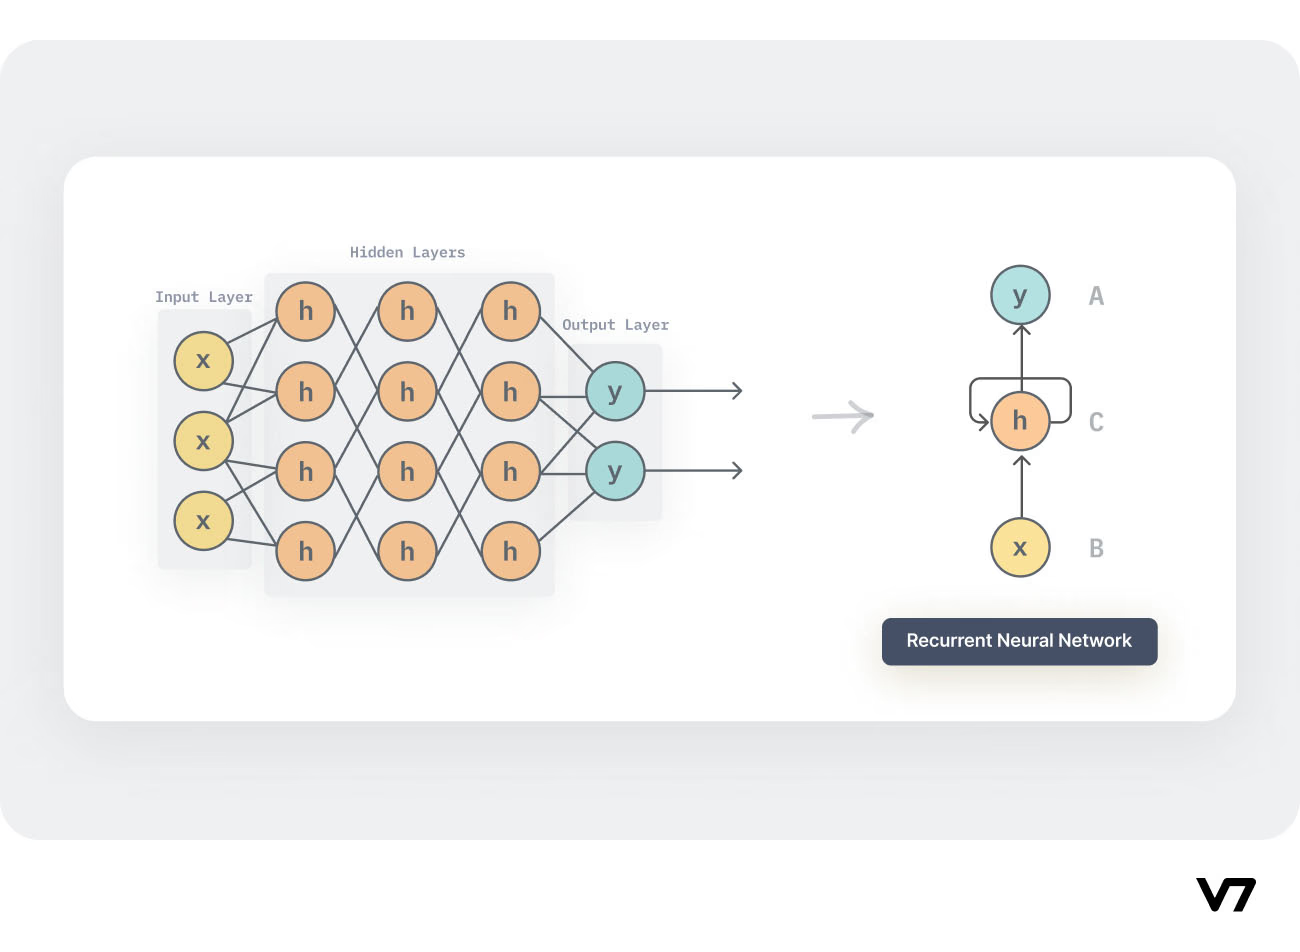
\includegraphics[scale=0.25]{capas.png}
    \caption{Capas en una red neuronal.}
\end{figure}

Durante este proceso, las (RNN) tienden a enfrentarse a dos problemas, conocidos como gradientes de explosión y gradientes de desaparición.
Estos problemas se definen por el tamaño del gradiente, que es la pendiente de la función de pérdida a lo largo de la curva de error.
Cuando el gradiente es demasiado pequeño, sigue haciéndose más pequeño, actualizando los parámetros de peso hasta que se vuelven insignificantes, es decir, cuando eso ocurre, el algoritmo ya no está aprendiendo.
La explosión de gradientes sucede cuando el gradiente es demasiado grande, lo que crea un modelo inestable.
En este caso, los pesos del modelo crecerán demasiado y, finalmente, se representarán como \textit{NaN}.
Una solución a estos problemas es reducir el número de capas ocultas de la red neuronal, lo que elimina parte de la complejidad de los modelos (RNN).

\begin{figure}[H]
    \centering
    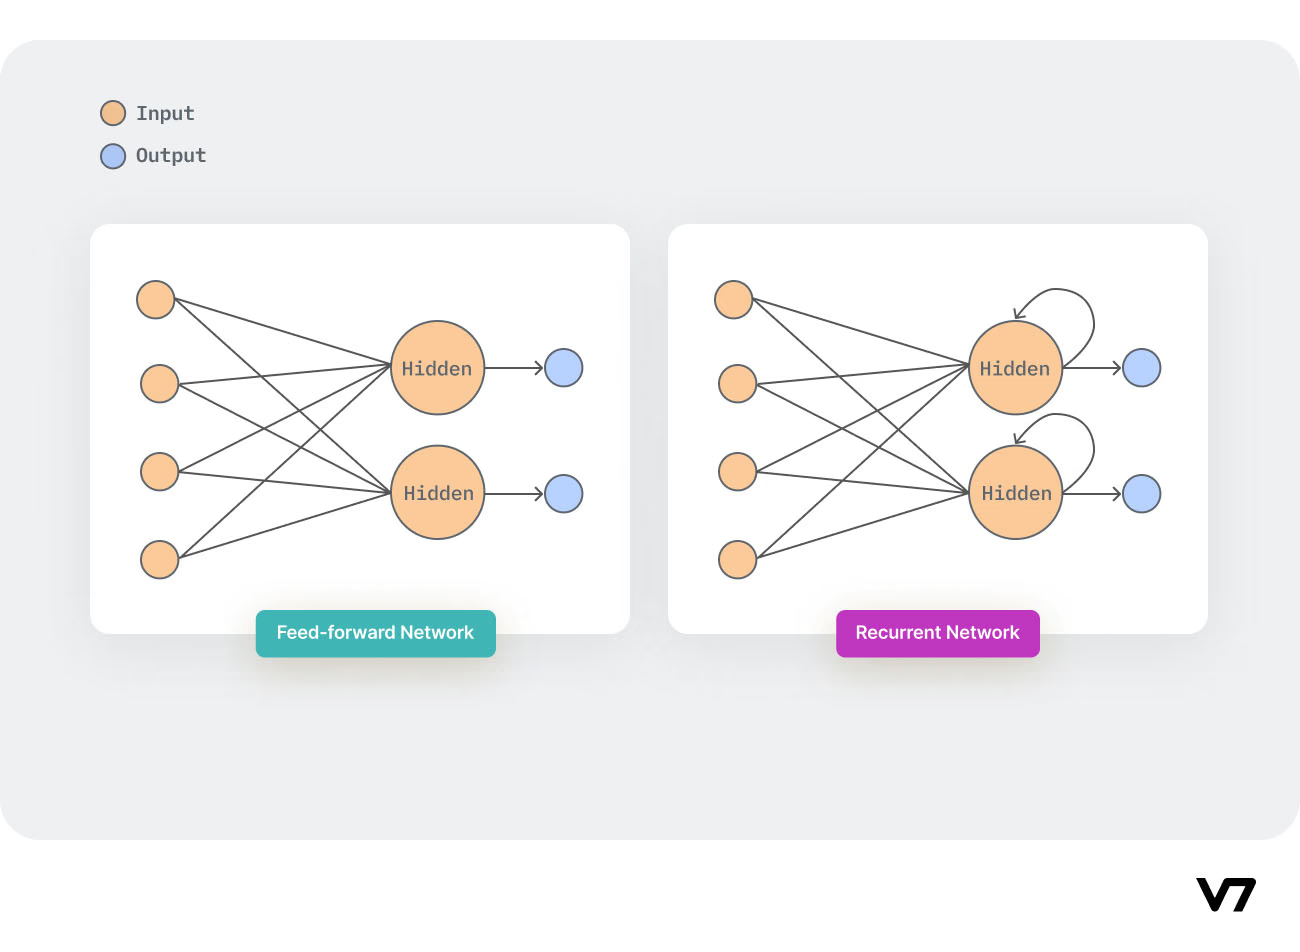
\includegraphics[scale=0.25]{ffrn.png}
    \caption{Feed-Forward Network vs Recurrent Network.}
\end{figure}

\newpage

\subsubsection{Tipos de RNN: Vanilla, LSTM, GRU, Bidireccional}
Las redes neuronales tradicionales tienen capas de entrada y salida independientes, lo que las hace inadecuadas para manejar datos secuenciales.
Las Redes Neuronales Recurrentes (RNN) se introdujeron para almacenar los resultados de salidas previas en una memoria interna.
Los cuatro tipos más comúnmente utilizados de Redes Neuronales Recurrentes son:

\begin{itemize}
    \item \textbf{One-To-One}: El tipo más simple de (RNN) es el One-to-One, que permite una sola entrada y una sola salida. Tiene tamaños de entrada y salida fijos, y actúa como una red neuronal estándar. Una de las aplicaciones del modelo One-to-One se encuentra en la clasificación de imágenes.
\end{itemize}

\begin{figure}[H]
    \centering
    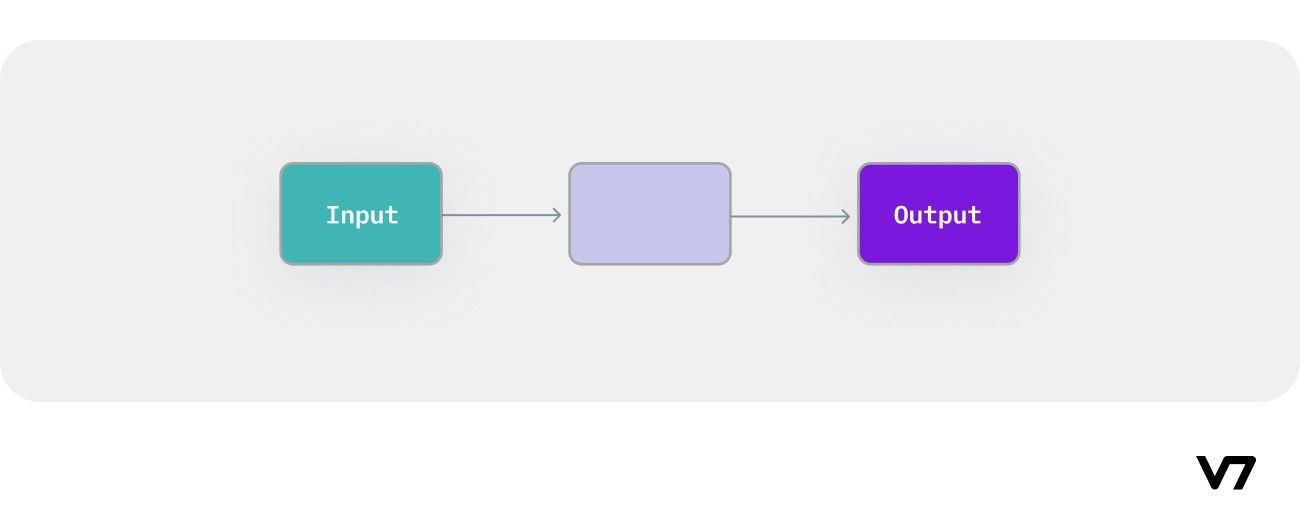
\includegraphics[scale=0.25]{oto.jpeg}
    \caption{One-To-One.}
\end{figure}

\begin{itemize}
    \item \textbf{One-To-Many}: El One-to-Many es un tipo de (RNN) que genera múltiples salidas a partir de una única entrada proporcionada al modelo. El tamaño de la entrada es fijo y produce una serie de datos como salida. Sus aplicaciones se encuentran en áreas como la generación de música y la generación de descripciones para imágenes (Image Captioning).
\end{itemize}

\begin{figure}[H]
    \centering
    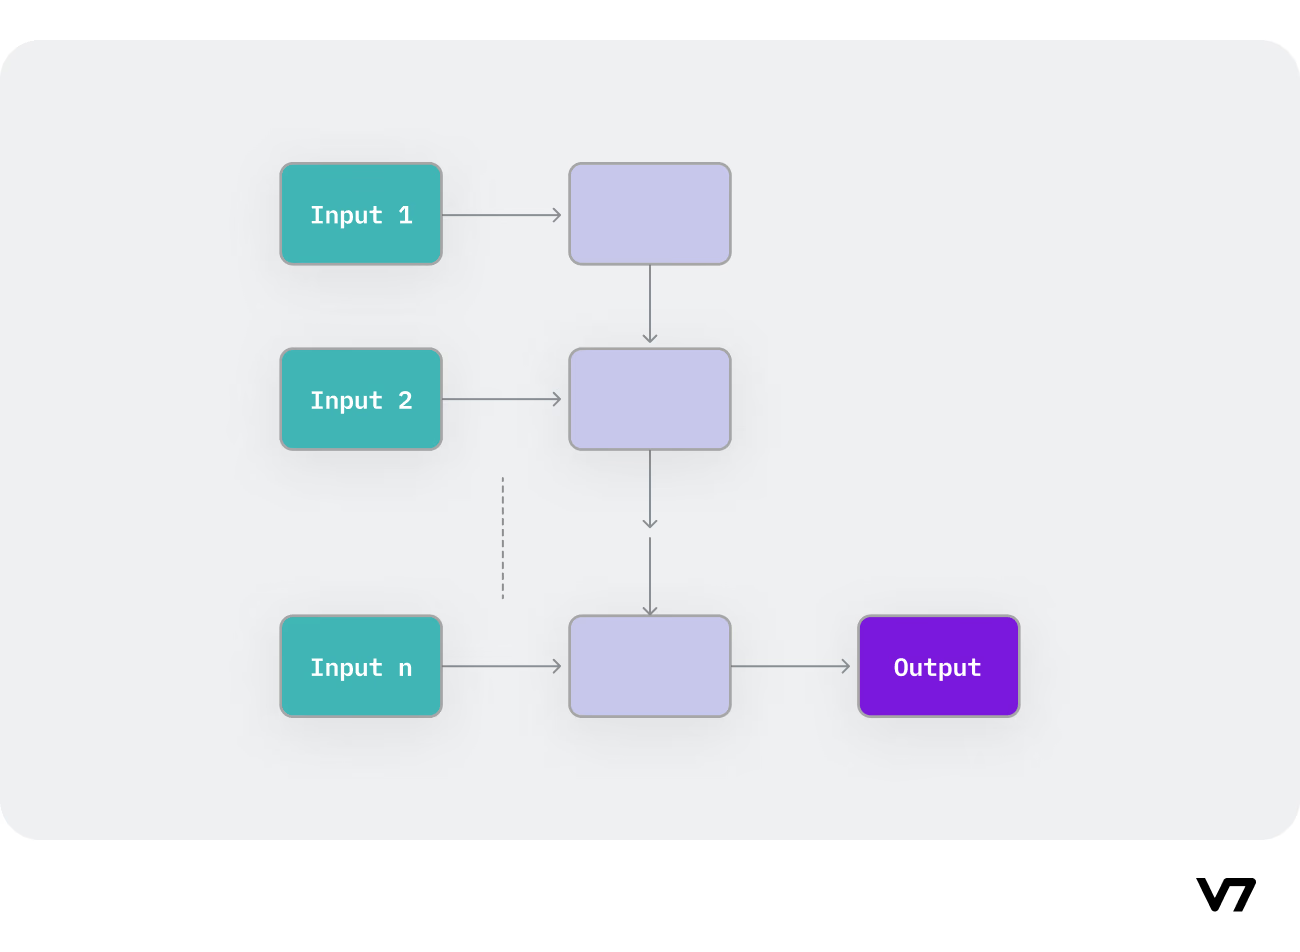
\includegraphics[scale=0.25]{mto.png}
    \caption{One-To-Many.}
\end{figure}

\newpage

\begin{itemize}
    \item \textbf{Many-To-Many}: es un tipo de RNN que se utiliza para generar una secuencia de datos de salida a partir de una secuencia de unidades de entrada. Este tipo se divide en las siguientes dos subcategorías:
\end{itemize}



\newpage
\subsubsection{Problemas de las RNN: Gradientes desvanecidos, Explosivos}

\subsection{Generación de Texto}
\subsubsection{Definición del problema}
\subsubsection{Flujo del modelo: tokenización, embeddings, RNN, decodificación}
\subsubsection{Métricas para evaluar el texto generado}

\subsection{Comparación con otros enfoques}
\subsubsection{RNN vs Transformers}

\subsection{Ventajas y Desventajas de las RNN}
\subsection{Problemas de las RNN}
\subsection{Aplicaciones de las RNN}
\subsubsection{Procesamiento del Lenguaje Natural (NLP)}
\subsubsection{Series Temporales}
\subsubsection{Reconocimiento de Voz}

\newpage

\section{Implementación Práctica}
\subsection{Preparación de Datos}
\subsubsection{Descarga y preprocesamiento del texto}
\subsubsection{Tokenización y codificación}
\subsubsection{Generación de ventanas (ventanas deslizantes)}

\subsection{Arquitectura del Modelo}
\subsubsection{Detalles de la arquitectura \texttt{CharRNN}: embeddings, LSTM, capa de salida}
\subsubsection{Hiperparámetros del modelo}
\subsubsection{Visualización de la arquitectura (diagrama opcional)}

\subsection{Entrenamiento}
\subsubsection{Configuración del entrenamiento (batch size, epochs, optimizador)}
\subsubsection{Función de pérdida y retropropagación}
\subsubsection{Monitoreo de métricas (pérdida de entrenamiento y validación)}

\subsection{Generación de Texto}
\subsubsection{Proceso de inferencia}
\subsubsection{Ajuste de la temperatura para variar la creatividad del texto generado}
\subsubsection{Ejemplos de texto generado}

\section{Resultados}
\subsection{Pérdida de entrenamiento y validación (gráficos de convergencia)}
\subsection{Ejemplos de texto generado}
\subsubsection{Texto inicial (épocas tempranas)}
\subsubsection{Texto final (épocas avanzadas)}
\subsection{Comparación con el estilo literario original (\textit{Don Quijote})}
\subsection{Observaciones sobre la coherencia del texto generado}

\newpage

\section{Conclusiones}
\subsection{Resumen de los resultados obtenidos}
\subsection{Fortalezas y limitaciones del modelo}
\subsection{Propuestas de mejora}
\subsubsection{Experimentar con GRU/LSTM más profundas}
\subsubsection{Uso de Transformers o más datos}

\section{Anexos}
\subsection{Código completo del proyecto (o enlace a un repositorio)}
\subsection{Explicación de cómo instalar y ejecutar el proyecto}
\subsubsection{Dependencias necesarias (PyTorch, tqdm, etc.)}
\subsubsection{Instrucciones para reproducir los resultados}
\subsection{Documentación adicional sobre métricas y técnicas utilizadas}

\newpage

\section{Bibliografía}
\nocite{*}
\printbibliography

\end{document}